% !TeX root = ../main.tex
\chapter{Numerical investigation}
\label{chapt:results}

\section{Perfomance of Conjugate Gradient on the GPU}

\section{Exracting quark masses}

The Dirac operator for Wilson fermions in the yukawa model is
\begin{equation*}
D_{n m}=\sum_\alpha\left[\frac{\gamma_\alpha \delta_{n+\alpha, m} - \gamma_\alpha \delta_{n-\alpha, m}}{2} + (m_q + g \phi) \, \delta_{n m}\right] .
\end{equation*}
In momentum space it reads
\begin{equation*}
\bar{D}_{f f^{\prime}}(p)=\left(m+ g \sigma \sum_\mu 2 \sin ^2\left(\frac{p_\mu}{2}\right)+i \sum_\mu \gamma_\mu \sin \left(p_\mu\right)\right) \delta_{f f^{\prime}}
\end{equation*}
The inverse can be checked to be 
\begin{equation*}
    \bar D_{f,f'} ^{-1} = \left[m + \dots\right] \ \left(m+ g \sigma \sum_\mu 2 \sin ^2\left(\frac{p_\mu}{2}\right) - i \sum_\mu \gamma_\mu \sin \left(p_\mu\right)\right) \delta_{f f^{\prime}}
\end{equation*}
One can now find the pole mass by imposing $D^{-1} = 0$ and gets 
\begin{equation*}
    m + \dots = 0
\end{equation*}

\section{Cooling with coloured noise}
In this section we report and discuss results of the Yukawa theiry using the technique of coloured noise to perform block-spin steps as outlined in the paragraph \ref{sec:coloured_noise}. We first set up the white noise simulation with $s=1$ on a lattice of size $8 \times 8$, with spacing $a$ and cutoff $\Lambda$. We then start performing complete block-spin steps as summarised in table \ref{tab:block_spin_steps}. \\


In the plots in figure \ref{fig:bs_NJL_quantities_mass}, reported as a function of the bare mesons mass. 
The peek in the magnetic susceptibility deserves some comment. In general, in a finite-volume lattice theory, no phase transition can happen. To state the presence of a phase transition, one should look at the infinite volume limit, which is done by studying the volume scaling of the magnetic susceptibility. In particular we do not expect a phase transition in our model due to the spontaneous breaking of the $O(1)$ symmetry, since the presence of a finite bare quark mass already breaks the $O(1)$ symmetry explicitly. As a remark to this statement, we studied the volume scaling of $\chi$, as reported in figure \ref{fig:chi_volume_scaling}. It is clear that it converges towards XXX, implying that the system is not undergoing a phase transition.

\begin{figure}
    \centering
    \begin{minipage}{0.45\textwidth}
        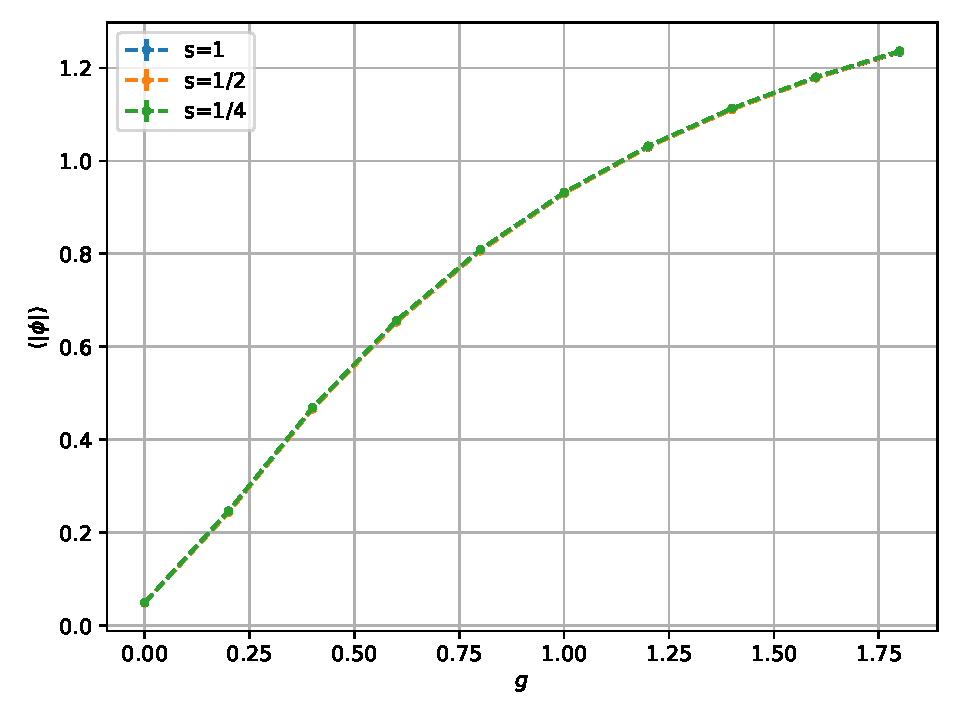
\includegraphics[scale=0.45]{figures/rescaling/magnetisation.pdf}
    \end{minipage}
    \hfill 
    \begin{minipage}{0.45\textwidth}
        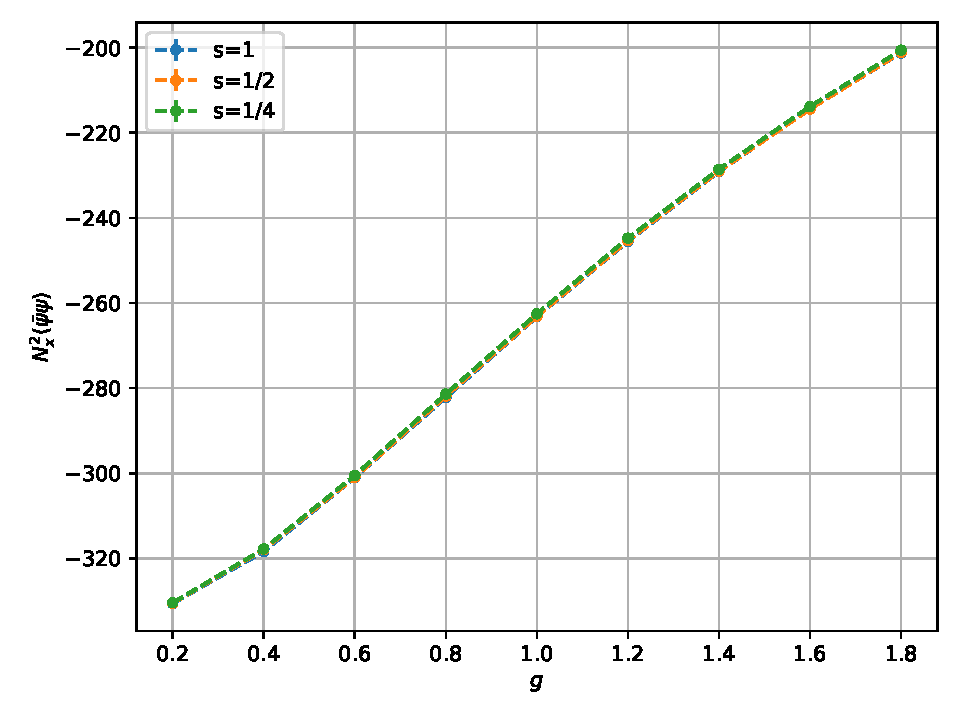
\includegraphics[scale=0.45]{figures/rescaling/condensate.pdf}
    \end{minipage}
    \begin{minipage}{0.45\textwidth}
        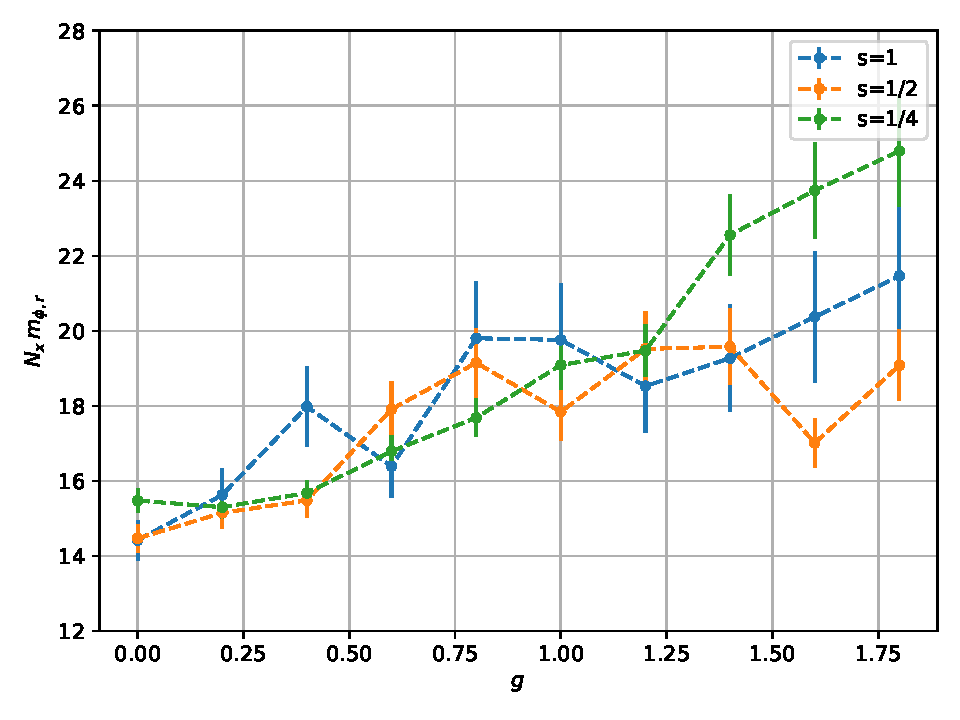
\includegraphics[scale=0.45]{figures/rescaling/mphir.pdf}
    \end{minipage}
    \hfill 
    \begin{minipage}{0.45\textwidth}
        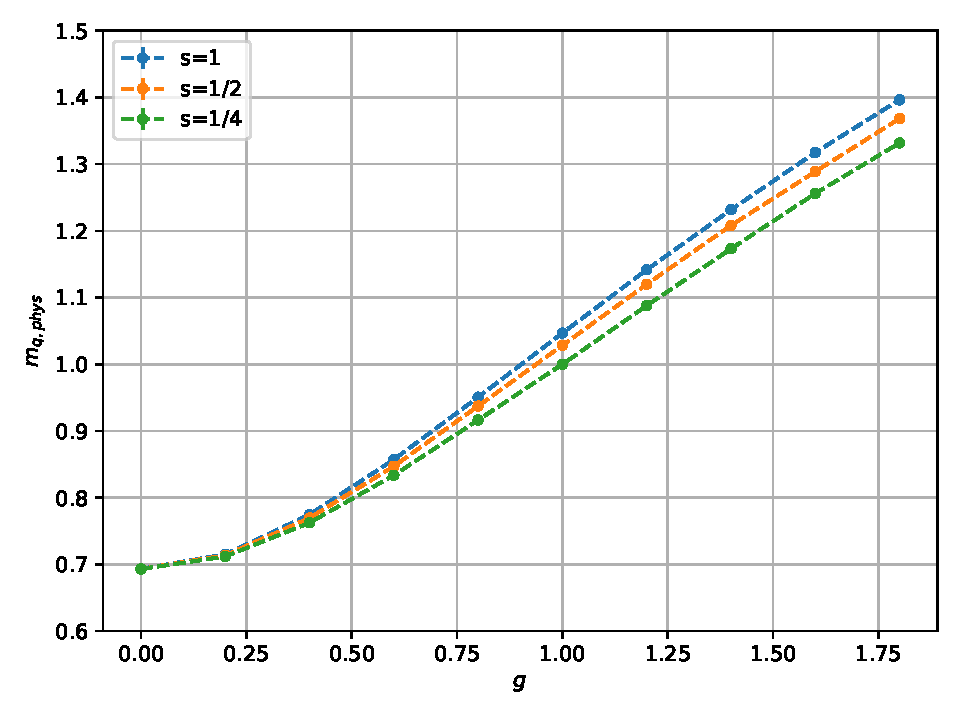
\includegraphics[scale=0.45]{figures/rescaling/mqphys.pdf}
    \end{minipage}
    \label{fig:cooling}
\end{figure}


Look at various things such as magnetization, mass, etc. \\
Even though is O(1) we do not observe SSB because of fermion bare quark mass. \\
Peak in the susceptibility does not imply P.T. $\rightarrow$ look at volume scaling. \\
When does L.O. rescaling ansatz breaks down?


\newpage

\begin{equation*}
    S[\phi, \bar\psi, \psi] = \int_x \phi \left(\frac{\partial^2}{2} + \frac{m_\phi^2}{2}\right) \phi + \frac{\lambda}{4!} \phi^4 + \bar \psi \left(\slashed{\partial} + m_q + g\phi\right) \psi
\end{equation*}

\begin{equation*} 
    \lambda = 1.0 \qquad m_\Phi^2 = 0.5 \qquad N_t \times N_x = 8 \times 32 \qquad m_q = 0.5 \qquad N_{conf} = 5 \cdot 10^3 \qquad \bar\epsilon = 0.01
\end{equation*}


\section{Classical to quantum interpolation}
\label{sec:classical_to_quantum}

Let us start by analising the coloured noise field in the simulation and relevant properties that emerge from it. We consider the Yukawa model described by the continuum action \ref{eq:yukaw_continuum}.
In figure \ref{fig:thermalisation_different_noise_fracs} the system is initialised in the same state for all the configurations, and then evolved with the Langevin equation with various noise fractions. The red line corresponds to the case $s=0$, namely a classical simulation. The blue line corresponds to the case $s=1$, namely the fully quantum case. As one can notice, the introduction of noise shifts the equilibrium expectation value of the field monotonically with the cutoff fraction: this is due to the fact that WHAT???. Note that a lower noise fraction is correlated to a faster convergence towards equilibrium. Moreover, low-distance fluctuations are suppressed due to the removal of the ultraviolet modes in the noise term.

For $\lambda = 0$ one has
\begin{equation}
    \sigma = -\frac{g}{m_\phi^2 + k^2} \, \bar\psi \psi
    \label{eq:equation_motion_NJL_no_self_interaction}
\end{equation}
In figure \ref{fig:equation_motion_NJL} one can see that equation \eqref{eq:equation_motion_NJL_no_self_interaction} is verified also on the fully quantum level.

Figures \ref{fig:slide_broken_phi} - \ref{fig:slide_broken_mphir} report a few observables as a function of the cutoff fraction $s$. In this case all the coupling constants are kept fixed while changing the value of $s$, in order to provide a smooth interpolation between the fully classical and fully quantum picture. \\
Each figure reports two plots corresponding to two different parameter configurations. The COLOR1 line corresponds to a system in the symmetric phase, while the COLOR2 line correspond to the broken phase. The exact parameters for the two configurations are reported under the figure.

\newpage
\section{Chiral fermions and a glimpse on the chiral phase transition}
\label{sec:chiral}

As explained in section \ref{sec:yukawa}, in the continuum theory chiral symmetry can be broken either explicitly via a finite bare quark mass, or spontaneously if the field gains a non-zero expectation value. Moreoveor, in the discrete formulation, the introduction of the Wilson term also contributes to the explicit breaking of chiral symmetry \textcolor{red}{add reference}, as explained in section \ref{sec:discrete}. This, in particular, means that chiral symmetry is explicitly broken also for $m_q \to 0$. Because of this, one needs a new definition for bare mass $M_q$, which takes into account the Wilson term contribution, such that chiral symmetry is restored in the limit $M_q \to 0$ for vanishing expectation value of the field $\phi$. A convenient way to define such $M_q$ is the following. SSB chiral symmetry $\to$ 3 goldstone massless bosons, the pions. If the bare quark mass is zero, the physical mass of the pions has to be zero. Hence one can extract this mass on the lattice and tune $m_q$ such that this is zero. While this is the correct way to proceed, it is very time takin since one must do mass scans and extrapolations close to singular Dirac operator. This is not the way we pursue here. Instead here we just consider naive fermions and take the limit $m_q \to 0$. This represents a physical theory with $2N_f = 4$ degenerate quarks. This is just done for the purpose of showing some interest properties of coloured noise and not (yet) to match any physical result. \\~\\
In figure \ref{fig:chiral_symmetry_breaking} some observables are reported as a function of the noise fraction $s$ for different values of the bare quark mass. In the classical theory ($s=0$) the order parameters $\left\langle|\phi|\right\rangle, \left\langle\bar\psi \psi\right\rangle$ are, in absolute value, bigger than in the quantum case ($s=1$).  As the chiral limit is approached $m_q \to 0$, the figure shows that the classical system lies in the broken phase, while in the quantum settings the symmetry is restored. \textcolor{red}{Discuss general phase structure looking at both $\phi$ and $\bar\psi\psi$}. One can see that as $m_q$ is reduced, the systems shifts from a crossover to a second order phase transition, ahighligthed by the susceptibility $\chi^2$ and the binder parameter $U_L$.

\textcolor{red}{This would be better discussed as a function of bare scalar mass:} \\
The difference gets more sharped as the base mass decreases, since the theory is closer to the chiral limit discussed above, which corresponds to the case $m_q=0$. In this limit the systems goes under a second phase transition, highlighted by a peak in the susceptibility and and abrubt change in the Binder cumulant. In contrast, for finite mass,  there is smooth crossover where the order parameters change continuously.

\begin{figure}[h]
\centering
\begin{minipage}{0.45\textwidth}	
	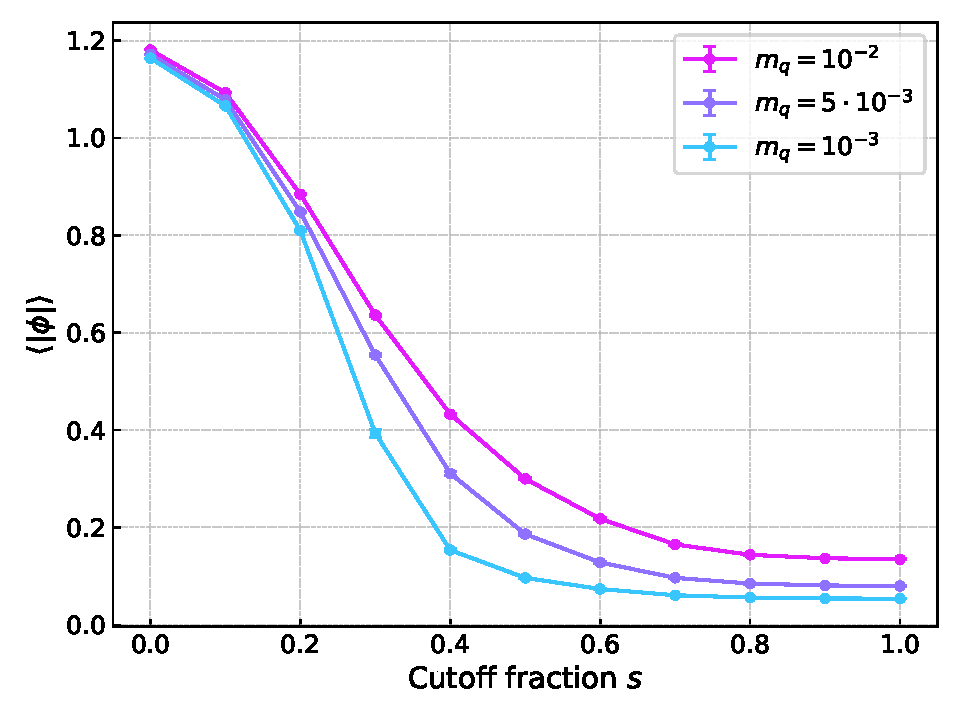
\includegraphics[scale=0.48]{figures/chiral_PT/magnetisation.pdf}
\end{minipage}
\hfill
\begin{minipage}{0.45\textwidth}	
	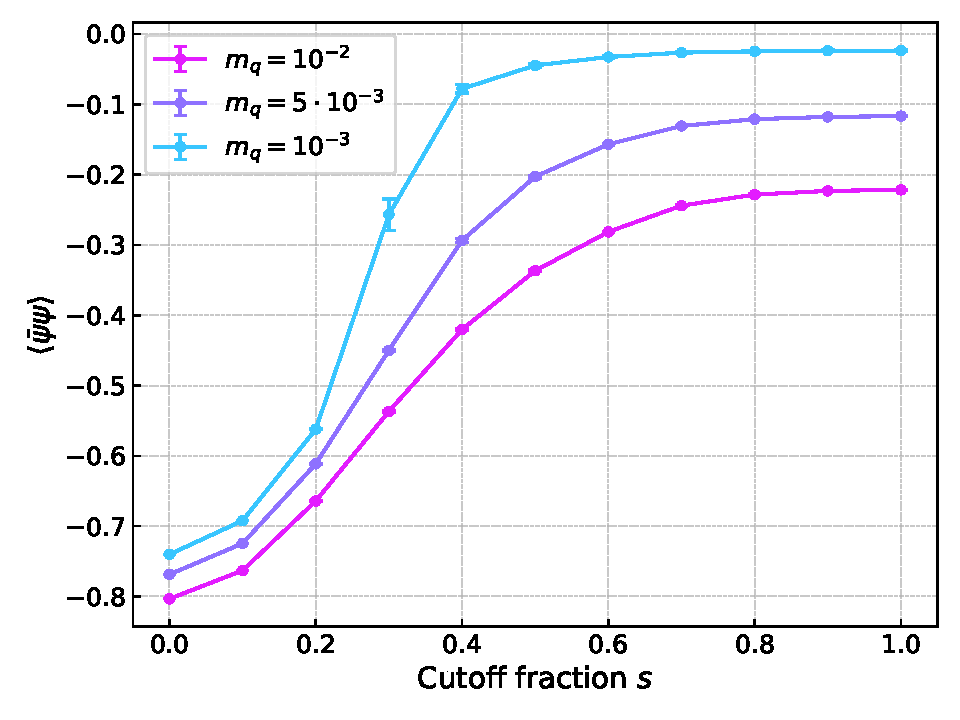
\includegraphics[scale=0.48]{figures/chiral_PT/condensate.pdf}
\end{minipage}
\begin{minipage}{0.45\textwidth}	
	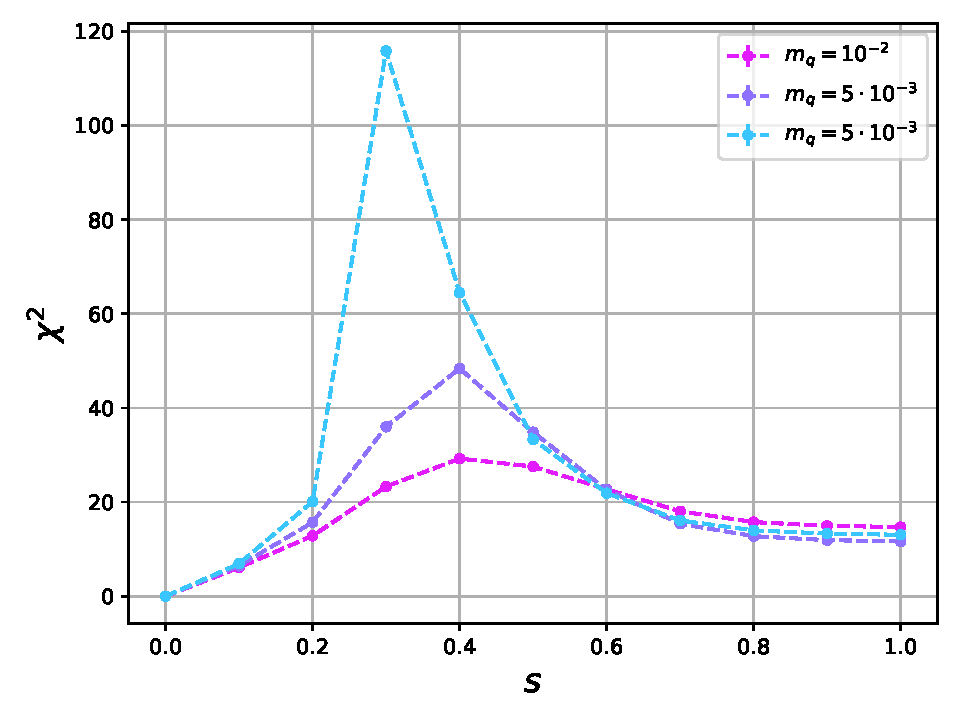
\includegraphics[scale=0.48]{figures/chiral_PT/susceptibility.pdf}
\end{minipage}
\hfill
\begin{minipage}{0.45\textwidth}	
	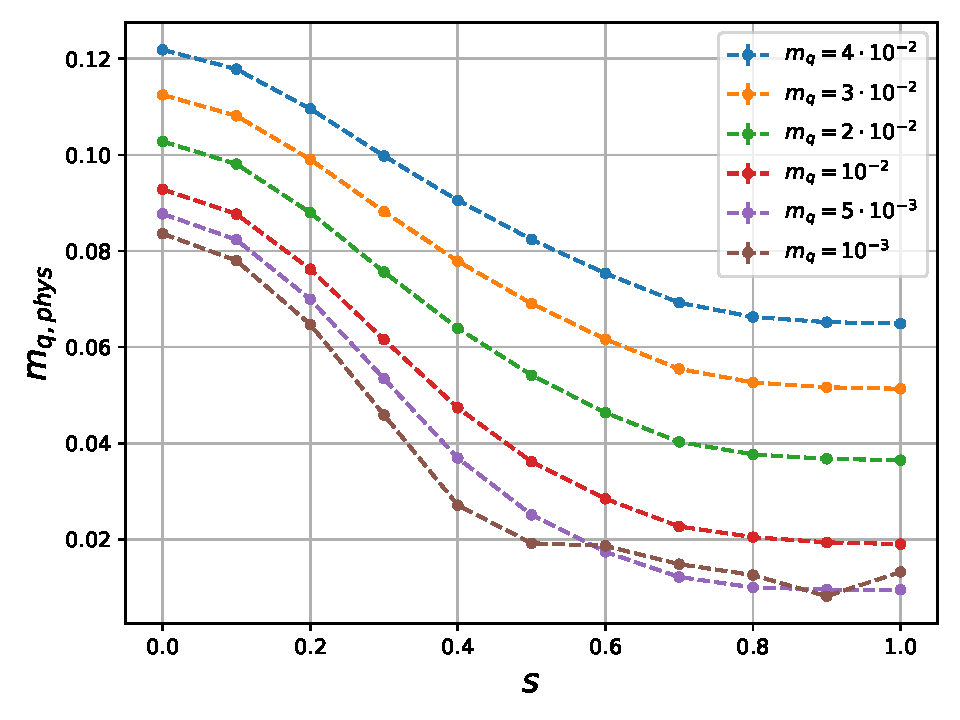
\includegraphics[scale=0.48]{figures/chiral_PT/mqphys.pdf}
\end{minipage}
\hfill
\begin{minipage}{0.45\textwidth}
	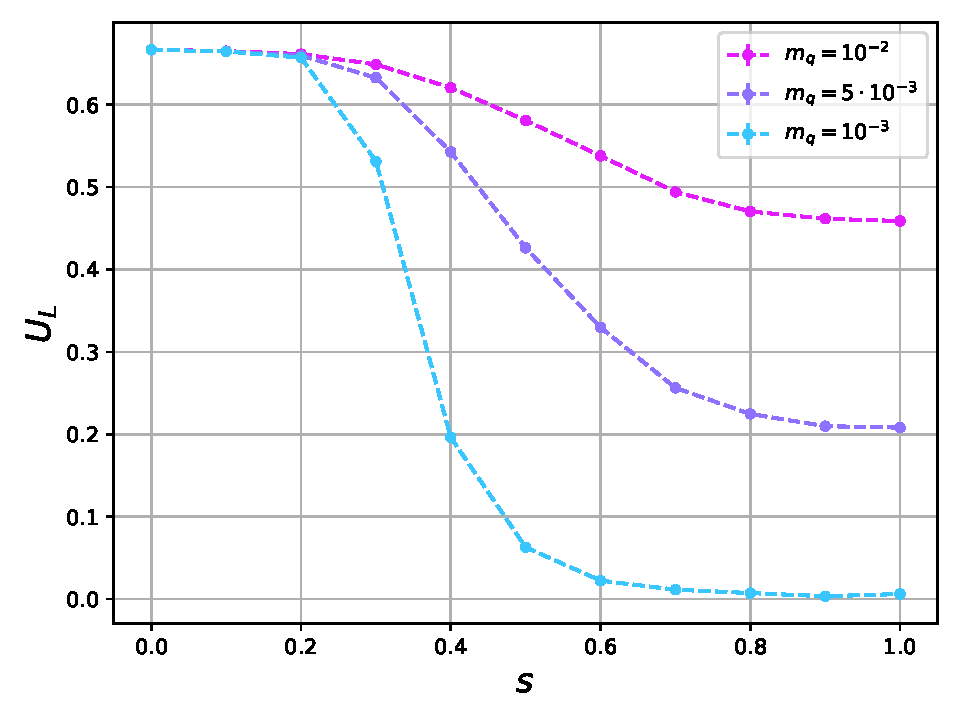
\includegraphics[scale=0.48]{figures/chiral_PT/binder.pdf}
\end{minipage}
\hfill
\caption{Chiral symmetry breaking}
\label{fig:chiral:symmetry_breaking}
\end{figure}


